\chapter{System Design}

The system design can be best explained with the help of this diagram: 

\begin{figure}[ht]
\begin{center}

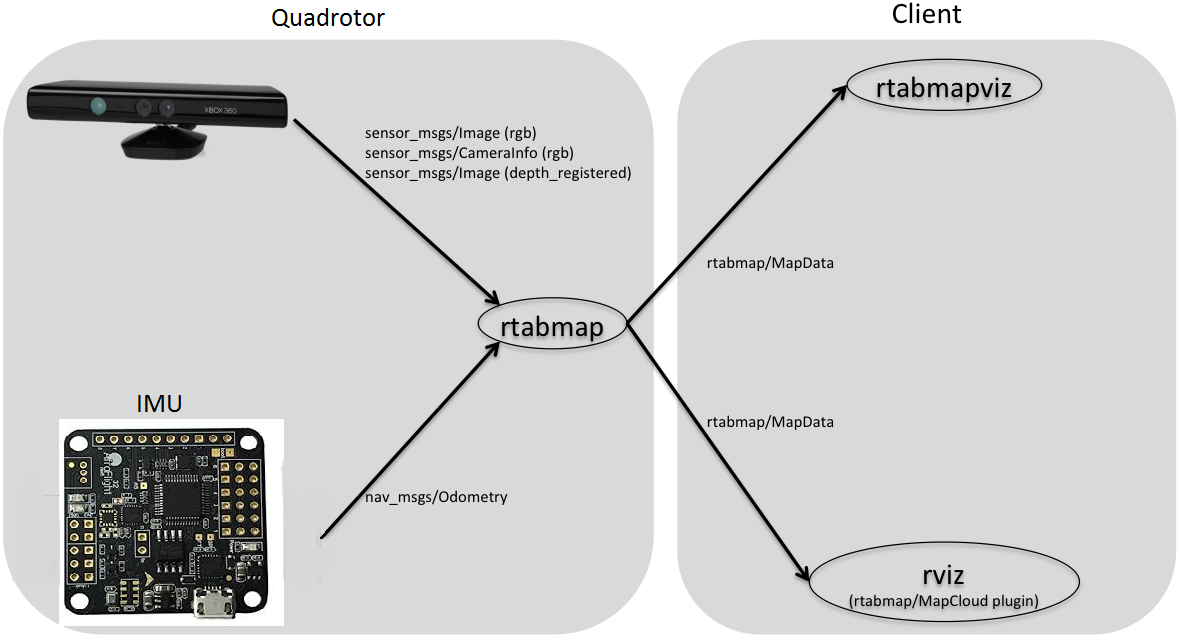
\includegraphics[scale=0.5]{setupC.png}

\captionsource{System Overview}{wiki.ros.org}

\label{fig:sys_overview}
\end{center}
\end{figure}

There are two systems running ROS, the onboard computer on the quadcopter and the base station computer(client). The quadcopter takes the depth data from the Kinect and the IMU data from the Flight Controller(FC), which is required for odometry, and sends it to RTAB-Map. Using these two critical data, RTAB-Map determines position of each point in the world forms a Map Cloud. This Map Cloud is obtained by the client computer over the ROS network and visualized in Rviz. 

\hspace{20pt}

Since this process involves many computations happening, transmitting the entire raw data would require a huge bandwidth and would not be feasible. Hence the data quality has to reduced and rate set to 5Hz to bring the bandwidth requirement to 80-120 kbps, which was measured using nethogs as seen in Figure \ref{fig:bandwidth}

\begin{figure}[ht]
\begin{center}

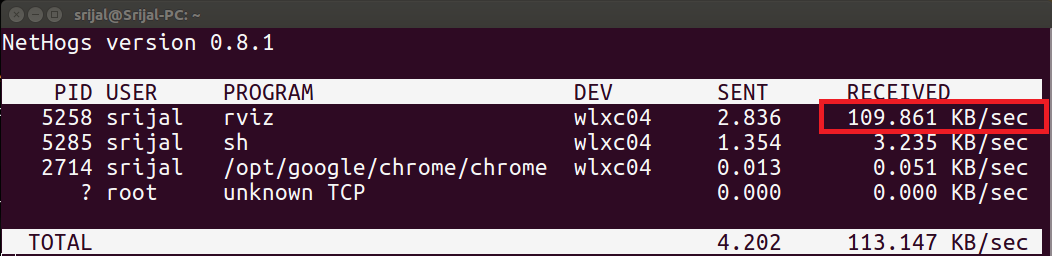
\includegraphics[scale=0.4]{ss1.png}

\caption{Bandwidth Requirement}

\label{fig:bandwidth}
\end{center}
\end{figure}


\begin{figure}[ht]
\begin{center}

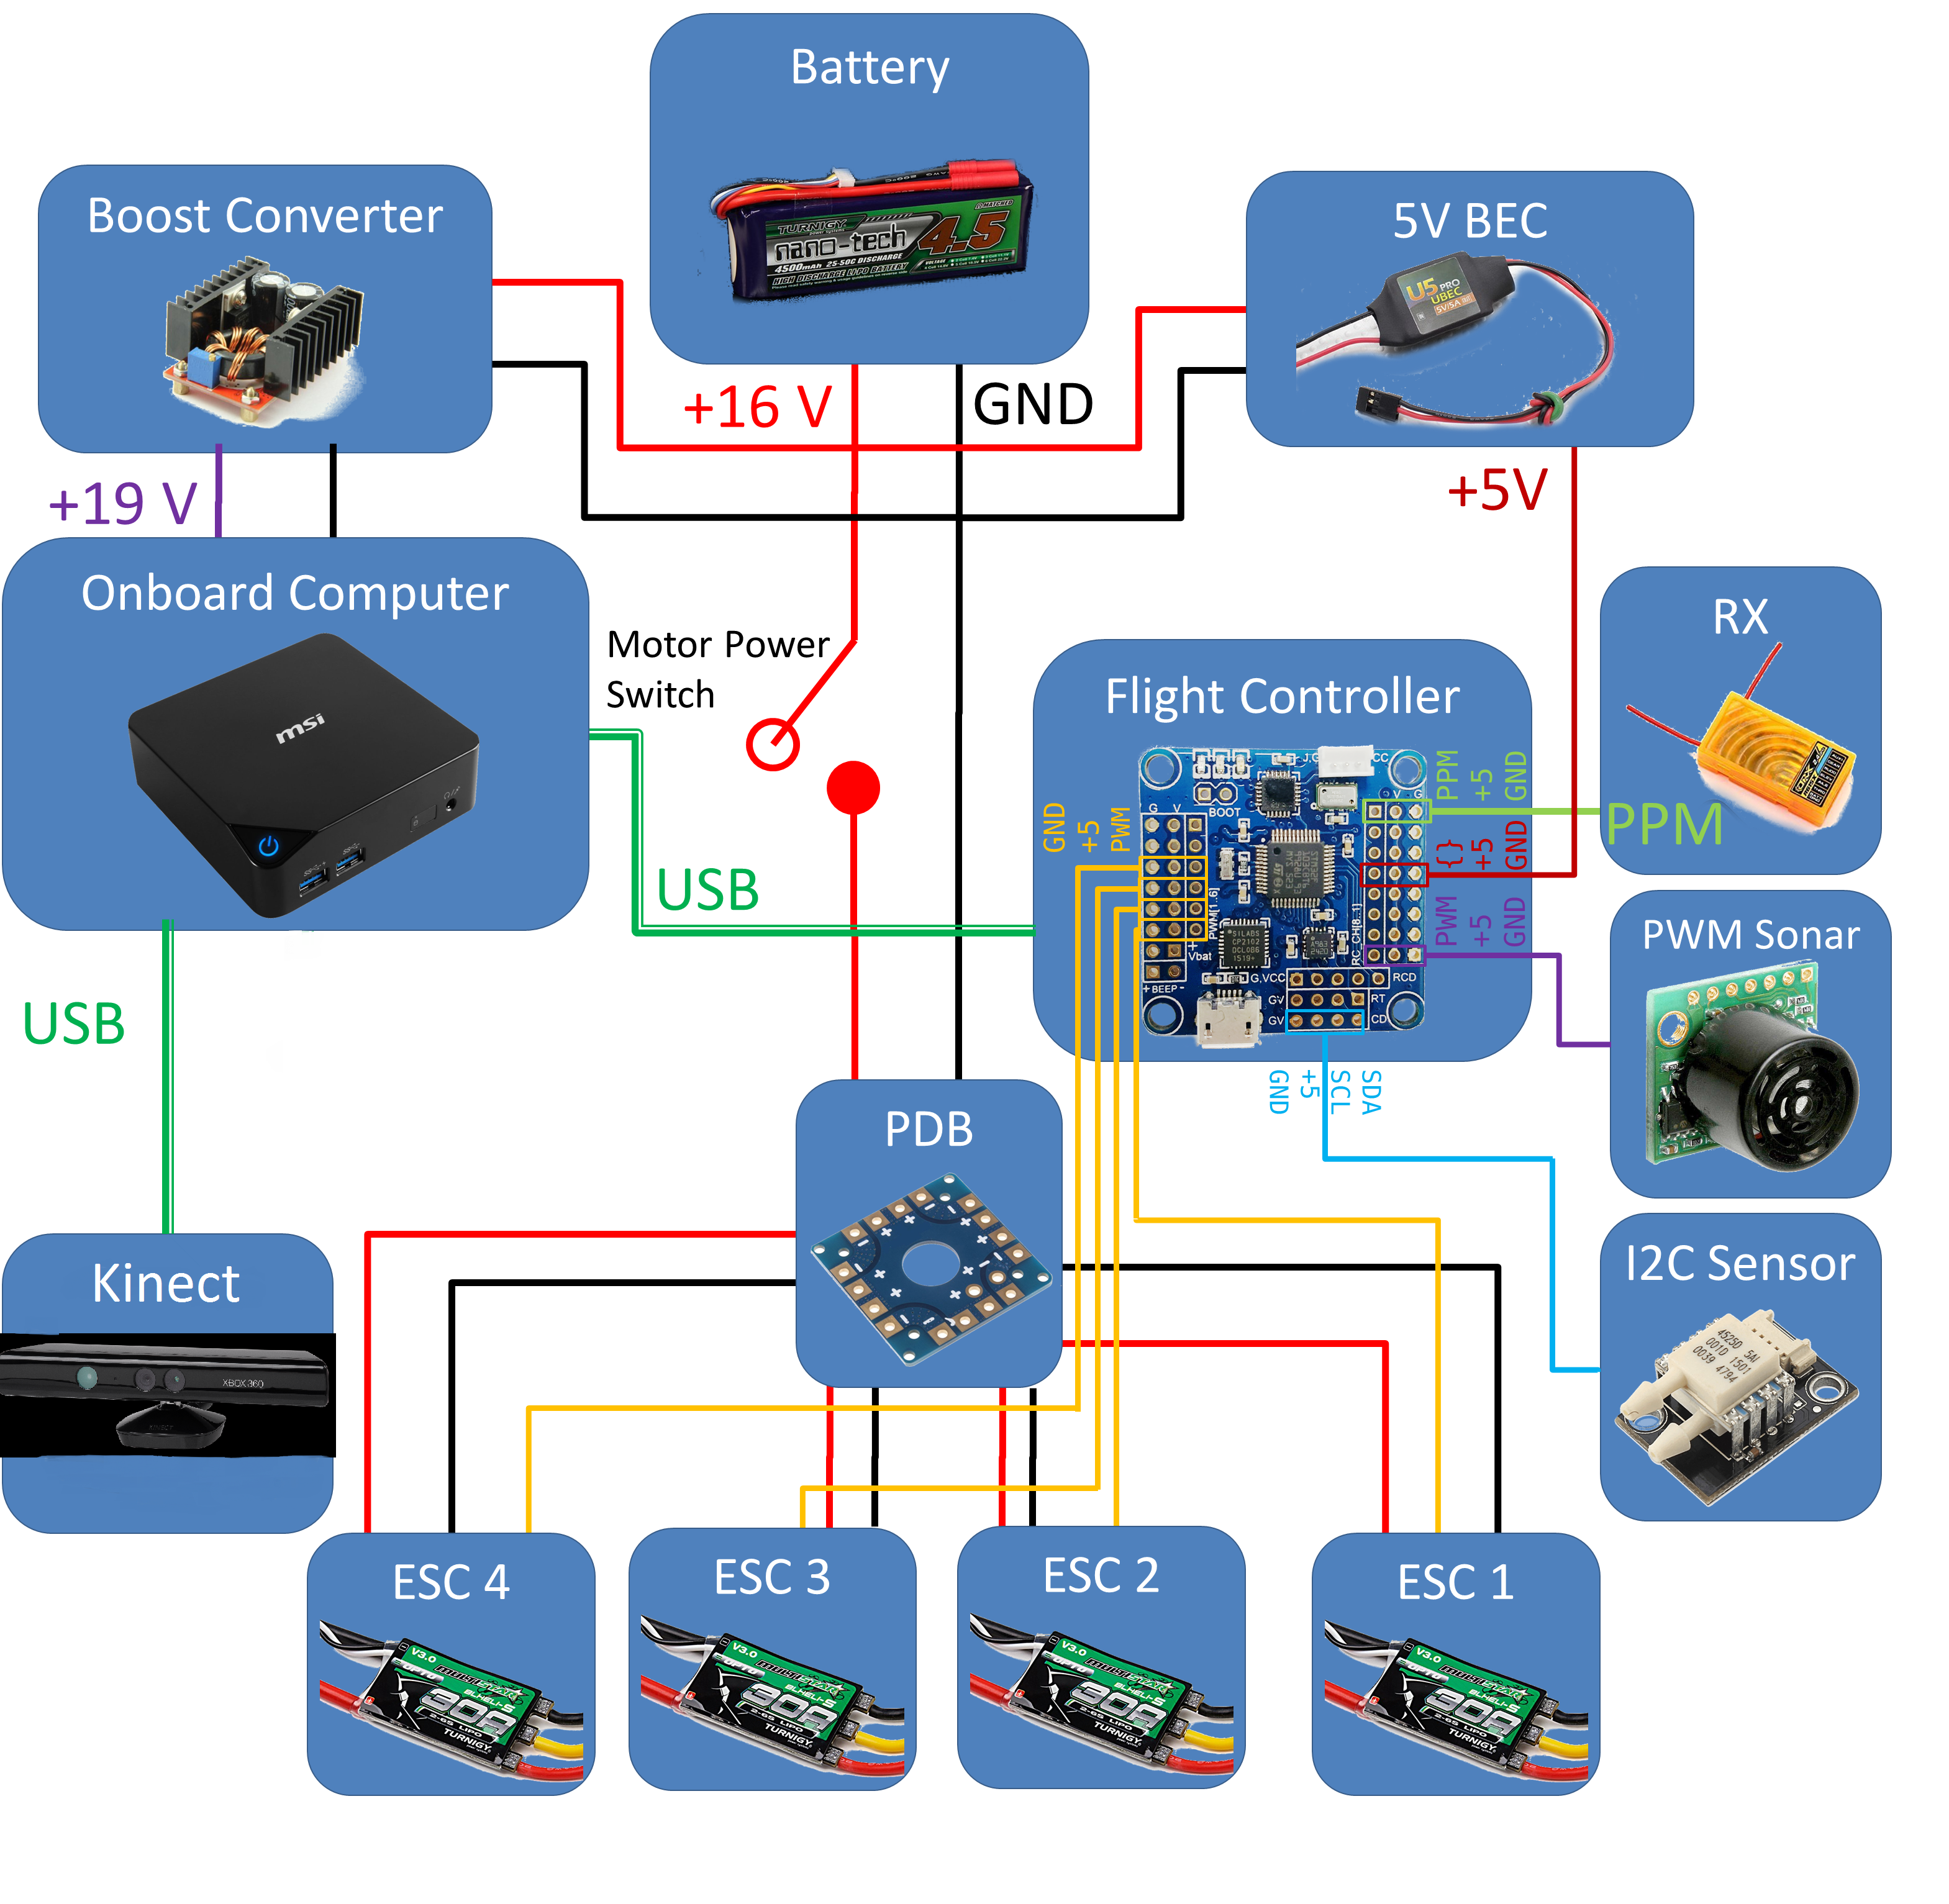
\includegraphics[scale=0.13]{Wiring_Diagram.png}

\captionsource{Quadcopter Hardware Layout}{docs.rosflight.org}

\label{fig:wiring}
\end{center}
\end{figure}

\vspace{20pt}

Since the onboard computer's terminal is not easily accessible, ssh is used by the client computer to issue the initial commands. 


